Figure \ref{fig:stx:concept} specifies the syntax used
to declare a \emph{concept}.
The \textbf{concept} keyword is followed by a NAME.
Optionally, a list of other NAMEs may be enumerated,
referring to other \emph{concepts}
that are generalizations (\ref{ch:generalization}) of the declared \emph{concept}.
A list of \emph{properties} (\ref{ch:properties}) may be declared under the \textbf{concept} block.
And the \textbf{abstract} keyword may precede the \textbf{concept} keyword, making a \emph{concept} abstract (\ref{ch:abstract}).

\begin{figure}
\verbatimfont{\small}
\lstinputlisting[language=antlr]{grammar/Concepts.txt}
\caption{Concept Declaration Syntax}
\label{fig:stx:concept}
\end{figure}

Figure \ref{fig:meta:concept} presents the \emph{concept} metamodel
in an EMOF \cite{mof} class diagram,
and figure \ref{fig:ast:concept} specifies
the \emph{concept} transformation
from its concrete syntax to its abstract syntax.
For each \emph{concept} parsed by the compiler,
an instance of the \emph{Concept} class will be created,
and its properties will be assigned
according to parsed information:

\begin{itemize}

\item \emph{name}:
assigned with the value of the terminal node NAME.

\item \emph{abstract}:
set to \emph{true} if the \textbf{abstract} keyword
is found before the \textbf{concept} keyword;
otherwise, set to \emph{false}.

\item \emph{elements}:
an \emph{ordered set} referencing all \emph{properties}
parsed in the \textbf{concept} block.

\item \emph{generalizations}:
an \emph{ordered set} referencing all \emph{concepts}
whose NAMEs were enumerated in the \emph{GeneralizationList}.

\end{itemize}

\begin{figure}
\centering
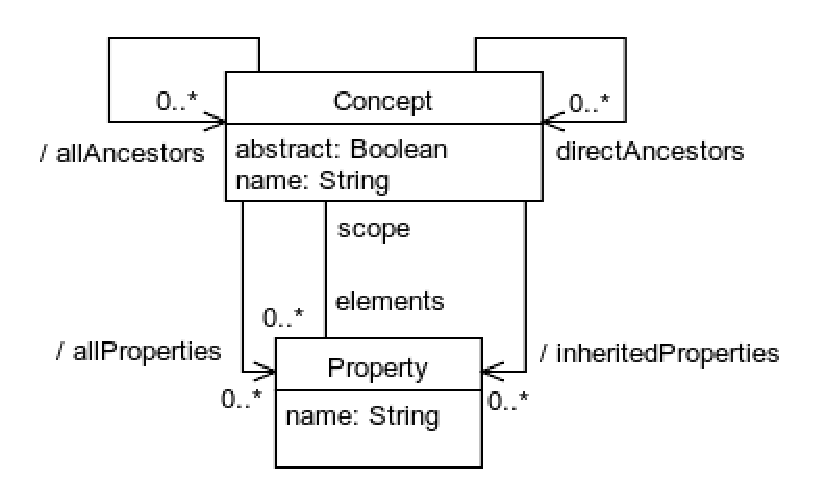
\includegraphics[width=0.5\textwidth]{metamodel/concept}
\caption{Concept Metamodel}
\label{fig:meta:concept}
\end{figure}

\begin{figure}
\verbatimfont{\small}
\lstinputlisting[language=lsl]{ast/concept.lsl}
\caption{Concept AST Instantiation}
\label{fig:ast:concept}
\end{figure}
